\section*{Implementation}

\subsection*{Previous Setup}

Before the start of the project, small programs were written in C++ and Python to analyze molecular data. The simulation data is provided in the form of an XML document (local or remote) that contains the full history of the molecular simulation. A separate Python script performed the extraction of the data from the XML document and a separate C++ program computed the radial distribution function. After the two programs were run, the user then had to use the GNUplot package to graph the radial distribution funciton. The overall setup can be described by the three blocks in the following diagram:

\begin{figure}[h]
\centering
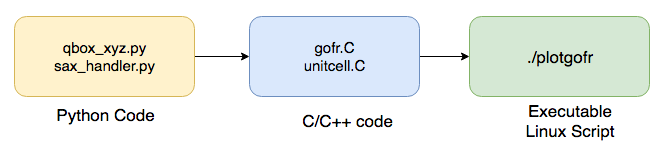
\includegraphics[scale=0.50]{images/old_pipeline}
\end{figure}

With respect to the above diagram, the following files performed the following functions: 

\begin{itemize}
        
    \item \verb|qbox_xyz.py|: Progressively parses the given XML document and only extracts the appropriate values defined in the \verb|sax_handler.py| XML handler. Handles the input data which is in XML format which contain details about the simulation, and outputs a file in .xyz format to be used by the \verb|gofr.C| C++ program.
    
    \item \verb|sax_handler.py|: This script stores the important data attributes required to extract data from the XML document for the radial distribution computation and visualization in the later phases.

    \item \verb|gofr.C|: A C++ program that performs the computation of the radial distribution function.
    
    \item \verb|unitcell.C|: Represents an abstraction of a unit cell (or simulation domain) defined by three basis vectors in three dimensional space.
    
    \item \verb|./plotgofr|: A linux executable shell script which visualizes the final output data using GNUplot.
    
\end{itemize}

One advantage of this approach was that the computation of the radial distribution function was very efficient. However, there were multiple problems with this approach:

\begin{itemize}
    \item Flexibility: This approach was not very flexible because a separate script had to be run during each phase of the process. In addition, the output data format was very similar to that of the GNU Plotting format, so if the user wanted to perform graphical analysis using a different software, it was a challenge.
    
    \item Usability: Since all these scripts used different languages and in some cases were platform dependent, integration was virtually absent. In other words, there was not one single platform which the user could run all the scripts but rather everything was split across different platforms and languages. In addition, the user had to switch between Python, C++, and bash scripts which could be inconvenient in some cases. 
    
    \item Interactivity: This was probably the biggest problem with the previous approach. The generation of the graphs was static in the sense that if the user wanted to visualize simulations of various sizes, the corresponding scripts would need to be run again and again for different configurations. In other words, there was not a way in which the user can \textit{interactively} examine and analyze the simulation data and visually examine how it would change over a period of time while the application was executing.
\end{itemize}

\subsection*{New Setup}
To eliminate most or all of the problems mentioned with the previous approach, a ``better'' solution was developed in terms of the scope of the project. Doing so involved developing and integrating all the scripts in one platform using one language. The main language of choice which was chosen during the development phase was Python. This was to make the scripts easier to run and also to make code extremely portable and usable. However, one downside with this approach was the performance of the calculation of the radial distribution function, which was the only bottleneck in the pipeline. (The performance issues will be discussed in later sections). The overall pipeline of the following project is as follows:

\begin{figure}[h]
\centering
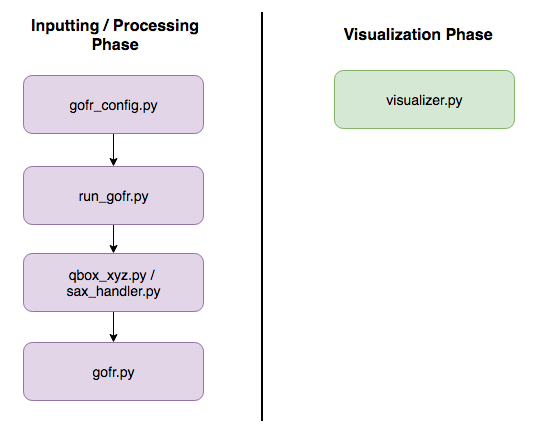
\includegraphics[scale=0.60]{images/new_pipeline}\newline
\end{figure}

With respect to the new setup, the following files perform the following functions: 

\begin{itemize}
        
    \item \verb|qbox_xyz.py|: Mostly remains unchanged with respect to the previous setup.
    
    \item \verb|sax_handler.py|: Also mostly remains unchanged with respect to the previous setup.

    \item \verb|gofr.py|: Computes the radial distribution function and the probability density functions. This file represents the translation of the C++ gofr.C code to python code. 
    
    \item \verb|unitcell.py|: Represents an abstraction of a unit cell, however the code is written in Python.
    
    \item \verb|run_gofr.py|: Runs the main gofr.py with the given inputs.

    \item \verb|visualizer.py|: This file generates a \verb|.html| page for interactive visualization of the pair distribution function.
    
\end{itemize}



\subsection*{Transition from C++ code to Python code}


\textbf{Differences}

Even though most of the functionality can be replicated and translated well in Python from C++, there are a few distinctions to be made. For instance, the operator overloading feature in C++ is a common practice whereas higher level languages such as Python or Java use function calls to replicate the effect. This was indeed the case with files such as \verb|unitcell.py|. In the C++ code, operators such as / (division), * (multiplication), etc were overloaded for vectors whereas the Python code achieved the same effect using function calls such as \verb|scalarProduct()| , \verb|length()|, etc.

Some other difference with the Python code was making the scripts as modular as possible in order to debug and create an efficient and a clean pipeline. Doing so not only improves code readability but is also easy to maintain. 

\textbf{Similarities}

The C++ code and Python code have a lot of similarities, especially for files such as \verb|UnitCell| and \verb|gofr|. The code and logic were mostly translated line by line from C++ and Python, and therefore the name of function calls and the constructors have also been provided the same names. The Object-Oriented paradigm has also been preserved across the translation and therefore the \verb|UnitCell.py| and \verb|Gofr.py| have corresponding constructors along with getters and setters. 

\subsection*{Performance Issues during translation}

The biggest challenge encountered was the performance of the radial distribution algorithm in Python. In short, this algorithm has a $O(n^2)$ time complexity for $n$ particles.  

\singlespacing
\begin{minted}{python}
 for i in range(species_1_count):
    for j in range(species_2_count):
      first_vector = tau[isp1[i]]
      second_vector = tau[isp2[j]]
      
      difference_vector = [ai - bi 
      for ai, bi in zip(first_vector, second_vector)]
      difference_vector = uc.fold_in_ws(difference_vector)
      scaled_vec = [x / dr for x in difference_vector]
      
      length_scaled_vec = sqrt(scaled_vec[0] ** 2 
      + scaled_vec[1] ** 2 + scaled_vec[2] ** 2)
     
      k = (int) (length_scaled_vec + 0.5)
      if k < nbin:
        count[k] += 1
\end{minted}

\doublespacing
In terms of functionalities, both pieces of code produce the correct results, however they vary significantly in performance. For instance, running the C++ code on $2,000$ time steps takes about $50$ seconds, whereas the corresponding Python code takes $15$ mins! This is due to the nature of the interpreted language and restrictions to manipulations at lower levels. In addition, the C++ code can be precompiled with some optimizations depending on the platform, which yields efficient results. In summary, the differences in performance can be highlighted in the following table:

\begin{center}
\begin{tabular}{ |c|c|c| } 
\hline
 Size of simulation (size of atomsets) &  Execution Time in C++ &  Execution Time in Python  \\
 \hline
 $20$ & $5$ sec & $9$ sec \\ 
 \hline
 $2000$ & $50$ sec & $15$ \textit{mins} \\ 
 \hline
 $10,000$ & $2$ min $10$ sec & $1$ hr $8$ mins \\ 
 \hline
\end{tabular}
\end{center}


\subsection*{New Features Added}

\begin{itemize}

\item Stepsize: Several new features were added during the translation. For instance, the precomputed radial function values can be stored every $n^{th}$ step, where $n$ can be adjusted by the user. By doing so, the size of the data stored is considerably reduced. This coarse graining of the data is made possible by the fact that the pair distribution function changes slowly during the course of a simulation.

\item Visualization: The visualization was performed in Javascript and a corresponding Python script generated the \verb|html| page. In addition, the visualization was interactive and customizable according to the user's needs.

\end{itemize}

\subsection*{Customization}

To customize the application according to the user's needs, the application has a configuration file. In this file, there are various parameters which the user can adjust according to visualization preferences and data origin. (For more details of what the configuration looks like please refer to the next section).


